	\chapter{Contrôle}
	Le système est contrôlé par deux microcontrôleurs un \pic ainsi qu'un \dspic. Le \pic se charge de la communication avec le smartphone au travers du module Bluetooth, il utilise ensuite les informations reçues pour contrôler le servomoteur de direction et envoie les informations adéquates au \dspic. Celui ci gère la puissance du moteur Brushless, il pilote l'onduleur triphasé.%Ajouter lien vers partie consacré plus haut
		\section{Communication}
			\subsection{Vue d'ensemble}
				Dans notre système, nous disposons de plusieurs appareils \textit{intelligent}, le \pic , le \dspic et le smartphone, afin que l'on puisse profiter au maximum des capacités de chacun, ces éléments doivent communiquer entre eux.
				\subsubsection{Technologies utilisées}
				Nous utilisons plusieurs technologies de communication différentes entre chaque composant.
				\paragraph{Entre le \textit{Smartphone} et le \textit{Module Bluetooth}} Une liaison \textit{Bluetooth Low Nergal} est établie entre le le module Bluetooth HC-05 et le smartphone. Dans notre cas, le téléphone est dit \textit{master} tandis que le module est dit \textit{slave}.
				\paragraph{Entre le \textit{Module Bluetooth} et le \textit{\pic} } Pour communiquer entre le module Bluetooth HC-05 et le \pic, une liaison série est utilisé. Cette liaison utilise deux conducteurs de données appelés TX et RX. La communication s'effectue à un baud rate commun entre les deux appareils. Le port TX d'un appareil est connecté au port RX du second et inversement.
				\paragraph{Entre le \textit{\dspic} et le \textit{\pic}} Entre ces deux composants, nous utilisons une connexion de type \textbf{SPI}. Cette liaison utilise 3 ou 4 conducteurs. Ils sont appelés SLCK (\textsf{Serial Clock}), MISO (\textsf{Master Input Slave Output}), MOSI (\textsf{Master Output Slave Input})  et SS (\textsf{Slave Select}). Le dernier n'étant utile uniquement si il y a plusieurs \textit{slave} dans le système. Dans notre cas, le \pic est \textit{master} et le \dspic est \textit{slave}
				
				\setlength{\unitlength}{1mm}
\begin{figure}
	\begin{picture}(210,45)
	
		\multiput(15,20)(50,0){4}{\oval(30,10)}
		\put(115,40){\oval(30,10)}
		\put(115,25){\line(0,1){10}}	  
		\put(165,0){\oval(30,10)}	 
		\put(165,5){\line(0,1){10}}   
		\multiput(30,20)(50,0){3}{\line(1,0){20}}  
		
	    \put(3,19){Smartphone}
	    \put(59,19){HC-05}
	    \put(105,19){\pic}
	    \put(102,39){Servomoteur}
	    \put(152,19){\dspic}
	    \put(155,-1){Onduleur}
	    
	    \scriptsize
	    \put(34,16){Bluetooth}
	    \put(88,16){Série}
	    \put(140,16){SPI}
	    \put(36,22){<0-255>}
	    \put(85,22){<0-255>}
	    \put(135,22){<100-200>}
	    \put(117,29){PWM}
	    \put(167,9){PWM}
	\end{picture}
	\caption{Diagramme de communication}
\end{figure}
				\subsubsection{Protocole}
				Avant de mettre en place une communication, il faut définir le \textit{langage} dans le quel nous allons parler. Entre le Smartphone et le Module Bluetooth, nous envoyons un octet. Nous avons donc 256 valeurs pour échanger les informations de puissance, de direction et d'effets. Nous avons donc décidé qu'à chaque mise à jour des curseurs de contrôle, des boutons d'effet ou en cas d'overflow du timer de sécurité, un nombre entre 0 et 255 serait envoyé par Bluetooth. On peut donc résumer les différente significations dans le tableau \ref{protocol}.
\begin{table}[h]
	\begin{center}
	
	\begin{tabular}{cc}
		<0>       & Information de connexion \\
		<1>    	  & Non utilisé               \\
		<2-20>    & Contrôle de la direction  \\
		<21-99>   & Non utilisé               \\
		<100-200> & Contrôle de la puissance  \\
		<201-255> & Effets                   
	\end{tabular}
		\end{center}
	\caption{Correspondance entre les valeurs et les fonctions associées}
	\label{protocol}
\end{table}

			\subsection{Application}
			Afin de pouvoir utiliser notre propre protocole, défini ci dessous, et d'avoir notre propre interface graphique nous avons décider de créer notre application de A à N. Pour cela, nous avons utilisé l'outil développer par le MIT, \href{http://ai2.appinventor.mit.edu/}{MIT App Inventor}. Cette outils en ligne permet de créer avec des blocs de simples applications pour smartphone.
		\paragraph{Interface de connexion} Lorsque nous démarrons l'application, nous arrivons sur un écran qui scan et liste les différents périphériques Bluetooth Low Energy à proximité de notre smartphone. Cette vue reprend les éléments développés dans ce tutoriel \cite{tutoBLE} du MIT. Plusieurs options s'offrent à nous, le scan des périphérique ou la connexion à un des périphériques. Lorsque nous nous connectons à un périphérique, nous basculons sur l'écran de commande de l'aéroglisseur.
		\begin{figure}
			\begin{center}
				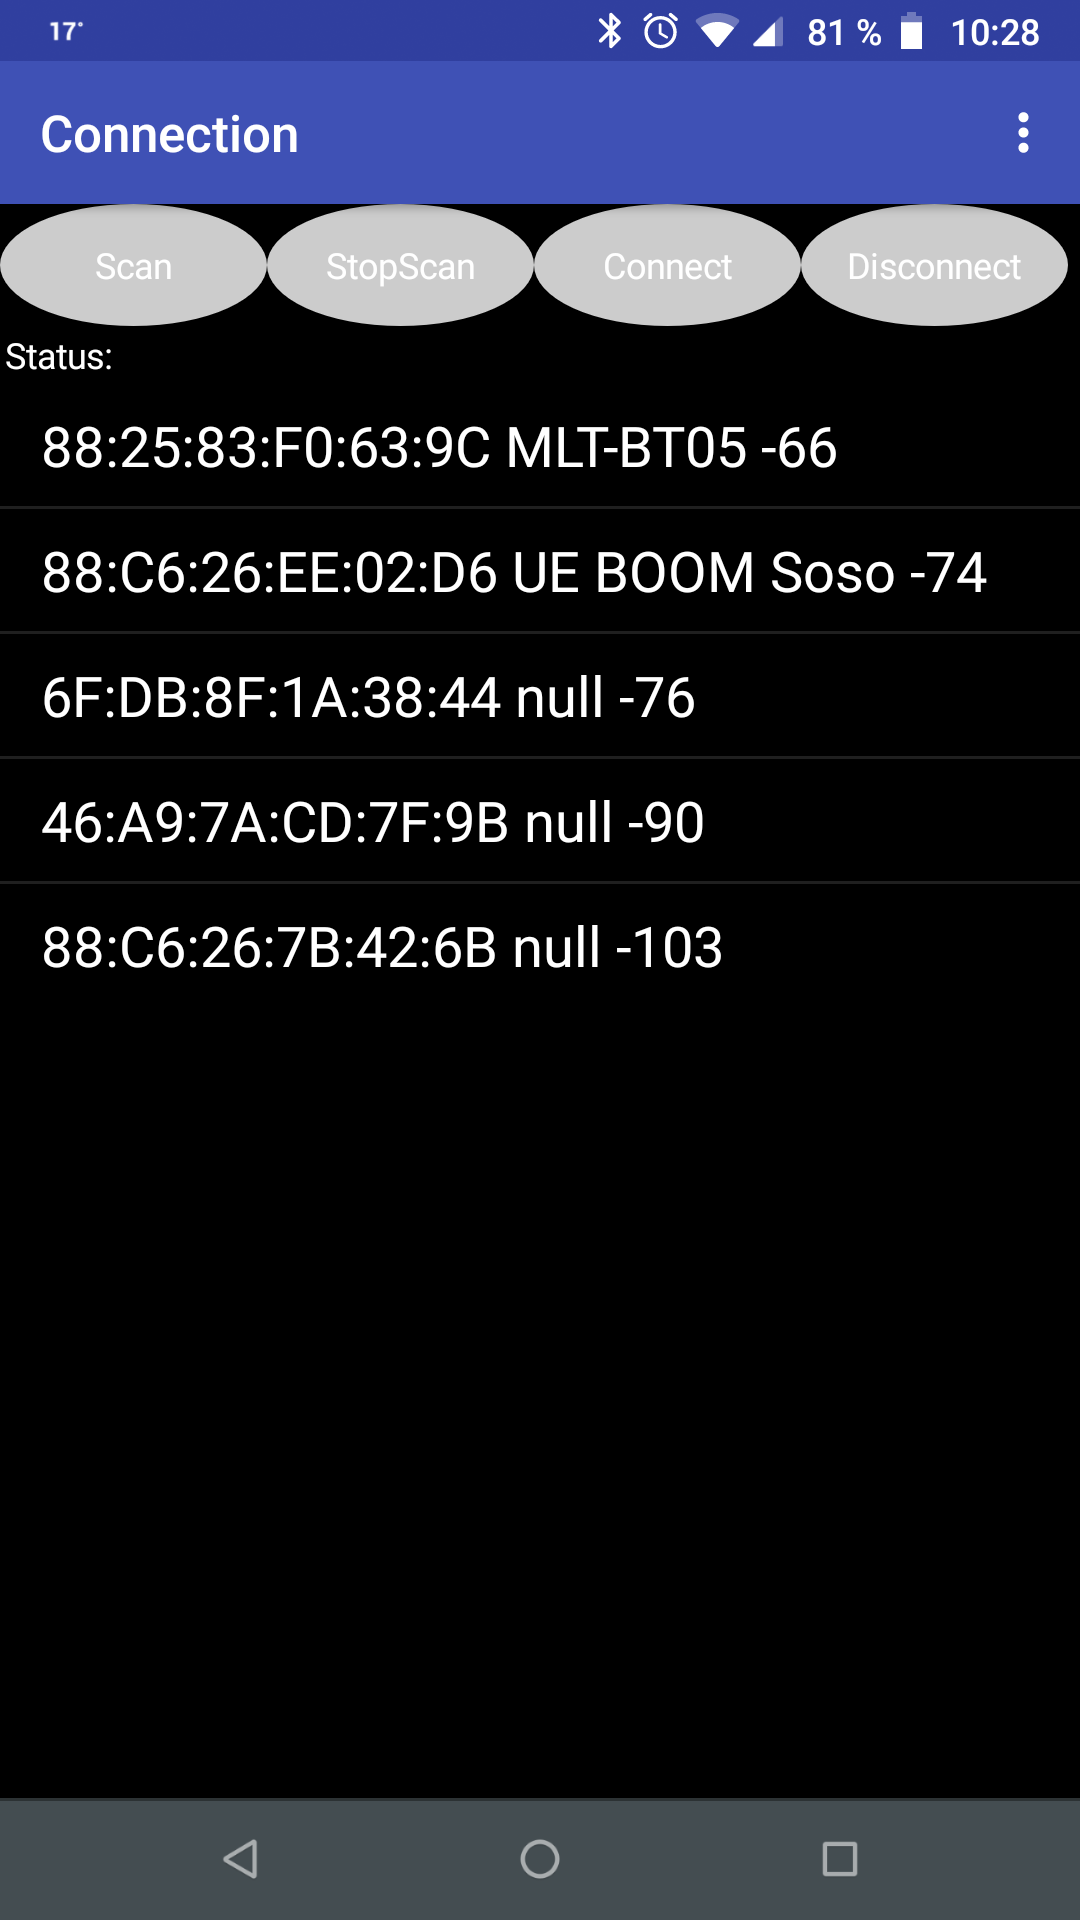
\includegraphics[width=0.3\textwidth]{../Illus/AppConnection.png}
			\end{center}
			\caption{Écran de connexion au périphérique Bluetooth}
		\end{figure}
			\paragraph{Interface de commande} L'écran de commande est composé de deux curseurs, celui de droite contrôlant la puissance et celui de gauche contrôlant la direction. En haut au milieu, il y a un bouton pour se déconnecter et revenir à l'écran d'accueil. En bas de l'écran, une série d'interrupteur permettant l'allumage de différents effets.
			\begin{figure}
		\begin{center}
			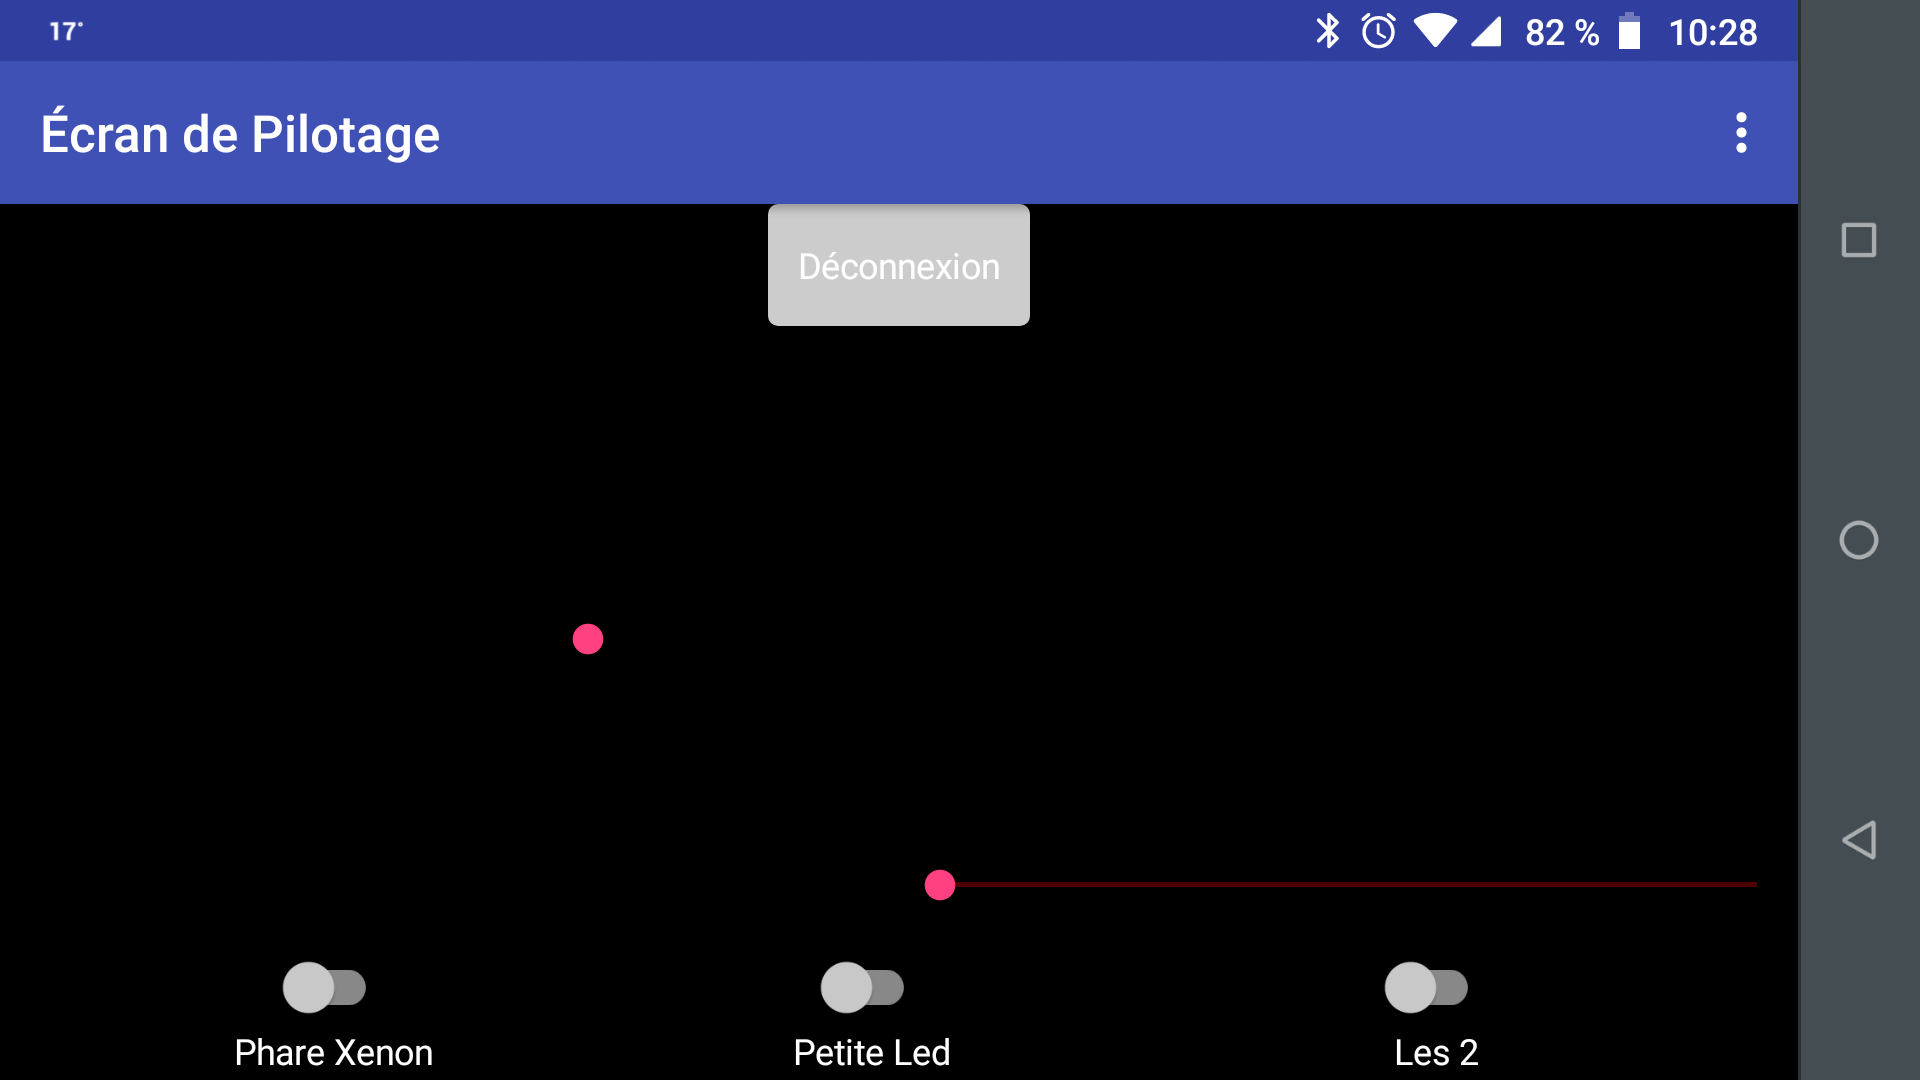
\includegraphics[width=0.6\textwidth]{../Illus/AppPilotage.png}
		\end{center}
			\caption{Écran de pilotage de l'aéroglisseur}
		\end{figure}
		\paragraph{Programmation}
		La programmation sur MIT App Inventor s'effectue avec des blocs. Chaque élément ajouté sur un écran est associé à des blocs fonctionnels. Cette manière de fonctionner ne permet pas de réaliser des applications extrêmement complexes mais permet de réaliser rapidement des interfaces sur smartphone. Notre application ne nécessite pas énormément de choses pour fonctionner, les écrans sont très simples. Nous pouvons résumer le fonctionnement de l'application avec le diagramme suivant.
		\begin{figure}
		\begin{picture}(500,120)
		\scriptsize
			\put(10,50){\framebox(25,10)[c]{\shortstack{Mouvement du\\ curseur Direction}}}
			\put(45,50){\framebox(25,10)[c]{\shortstack{Mouvement du\\ curseur Puissance}}}
			\put(80,50){\framebox(25,10)[c]{Appui sur un effet}}
			\put(115,50){\framebox(25,10)[c]{Fin du timer}}
			\put(150,50){\framebox(25,10)[c]{\shortstack{Appui sur\\ déconnexion}}}

			\put(92.5,80){\line(0,-1){10}}
			\put(22.5,70){\line(1,0){140}}			
		
			\multiput(22.5,50)(35,0){4}{\vector(0,-1){20}}
			\multiput(22.5,20)(35,0){4}{\vector(0,-1){10}}
			\multiput(22.5,70)(35,0){5}{\vector(0,-1){10}}
			\put(162.5,50){\line(0,-1){20}}			
			
			\put(162.5,30){\line(1,0){20}}
			\put(182.5,30){\line(0,1){90}}
			\put(0,10){\line(1,0){127.5}}			
			
			\put(0,75){\vector(1,0){92.5}}			
			
			\put(0,10){\line(0,1){65}}				
			
			\put(10,20){\framebox(25,10)[c]{\shortstack{Envoi de la valeur\\<2-20>}}}
			\put(45,20){\framebox(25,10)[c]{\shortstack{Envoi de la valeur\\<100-200>}}}
			\put(80,20){\framebox(25,10)[c]{\shortstack{Envoi de la valeur\\<201-255>}}}
			\put(115,20){\framebox(25,10)[c]{\shortstack{Envoi de la valeur\\<0>}}}

			
			\put(80,80){\framebox(25,10)[c]{\shortstack{Appui sur\\ connexion}}}
			
			\put(80,100){\framebox(25,10)[c]{\shortstack{Scan}}}
			\put(92.5,100){\vector(0,-1){10}}
			\put(92.5,120){\vector(0,-1){10}}
			\put(110,95){\line(0,1){20}}
			\put(92.5,95){\line(1,0){17.5}}
			\put(92.5,120){\line(1,0){90}}
			\put(92.5,115){\line(1,0){17.5}}
		\end{picture}
			\caption{Algorithme de fonctionnement de l'application}
			\label{algo}
		\end{figure}
		\\Chaque fonction ci dessus est assimilable à un bloc de MIT App Inventor. Par exemple, prenons la branche \textit{Mouvement curseur direction}.
		\begin{figure}
			\begin{center}		
				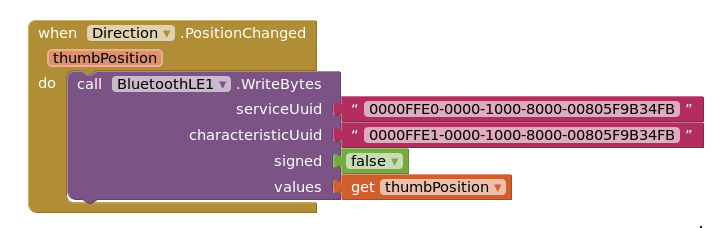
\includegraphics[width=0.5\textwidth]{../Illus/MITBlock.png}
				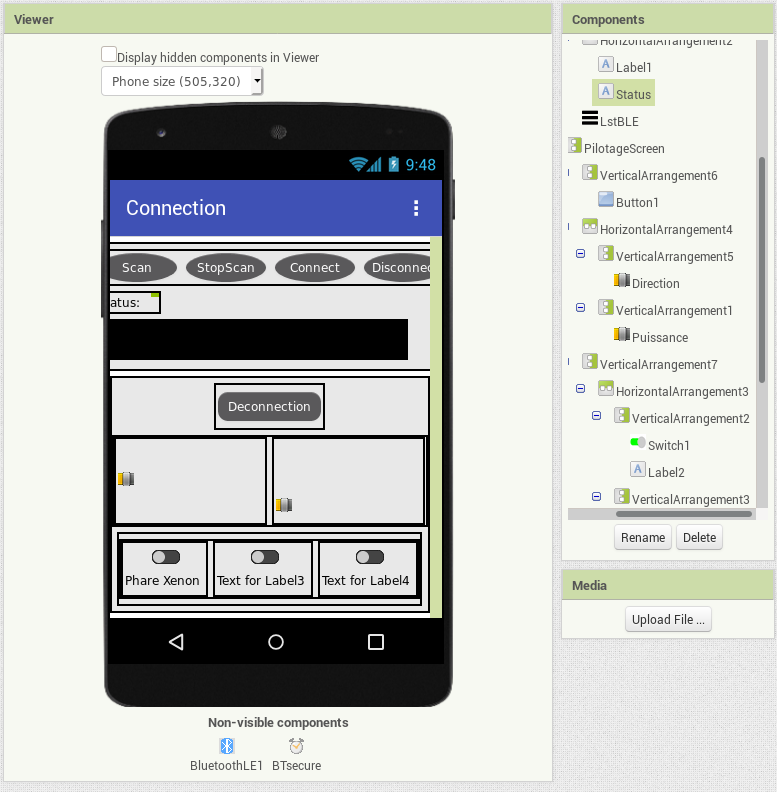
\includegraphics[width=0.275\textwidth]{../Illus/MITScreen.png}
			\end{center}
			\caption{Vues de MIT App Inventor}
		\end{figure}
		Nous pouvons voir les différents éléments constituant notre application, et un exemple de bloc qui réagit au changement de position du curseur pour l'envoyer le la liaison Bluetooth Low Energy.
		\\Les sources du projet de l'application est disponible sur notre dépôt Github ici\cite{git}.
			\subsection{Réception Bluetooth}
			Après avoir émis les informations de pilotage, il faut les récupérer pour les exploiter. Nous avons donc mis en place une liaison série entre le module Bluetooth HC-05 et le \pic. Cette liaison est déclarée à 9600 bauds.
			\paragraph{Mise en place}La configuration du module \textit{UART} du \pic est réalisée en s'appuyant sur la documentation technique\cite[p.~315]{DatasheetPIC}. On décide les pins que l'on va utiliser, tous les pins utilisés sur les microcontrôleurs sont précisés dans le tableau \ref{pinoutpic} et \ref{pinoutdspic}.
			
			\insertcode{../../ENUM/Codes/mainpic.c}{73-83,180-182,189-190}{Initialisation de la liaison série sur le \pic}
			
	
			\subsection{Liaison SPI}
			\insertcode{../../ENUM/Codes/mainpic.c}{96-107}{Initialisation de la liaison SPI sur le \pic}

		\section{Fonctionnement}
		Dans les tableaux \ref{pinoutdspic} et \ref{pinoutpic} sont réunis tous les pins utilisés sur chacun de nos microcontrôleurs.
		\begin{table}
			\begin{center}
				\begin{tabular}{r|ccc|l}
	
				VCC		& 1 &   & 20 & GND \\ 
				  		& 2 &   & 19 & PRGD \\ 
				 		& 3 &   & 18 & PRGC \\ 
				MCLR 	& 4 &   & 17 & Arrêt d'urgence \\ 
				Servo 	& 5 &   & 16 &   \\
				 Effet	& 6 &   & 15 &   \\ 
				  		& 7 &   & 14 & SDO \\ 
				  		& 8 &   & 13 & SDI \\ 
				BTTX 	& 9 &   & 12 & BTRX \\ 
				SCK 	& 10&   & 11 &   \\ 
				\end{tabular} 
			\end{center}
			\caption{Plan de branchement sur le \pic}
			\label{pinoutpic}
		\end{table}
		\begin{table}
			\begin{center}
				\begin{tabular}{r|ccc|l}
				MCLR 	& 1 &    & 28 & AVDD 	\\ 
				  		& 2 &    & 27 & AVCC 	\\ 
				  		& 3 &    & 26 &   		\\ 
				  		& 4 &    & 25 &  	 	\\ 
				  		& 5 &    & 24 & 		\\ 
				  		& 6 &    & 23 &   		\\ 
				 		& 7 &    & 22 &   		\\ 
				GND 	& 8 &    & 21 &   		\\ 
				  		& 9 &    & 20 & VDD 	\\ 
				  		& 10 &   & 19 & GND 	\\ 
				  		& 11 &   & 18 & SDI 	\\ 
				  		& 12 &   & 17 & SDO 	\\ 
				VDD 	& 13 &   & 16 & SCK 	\\ 
				  		& 14 &   & 15 &   		\\ 
				\end{tabular} 
			\end{center}
			\caption{Plan de branchement sur le \dspic}
			\label{pinoutdspic}
		\end{table}
			\subsection{Contrôle du servomoteur}
			\paragraph{Fonctionnement}
			Un servomoteur est un moteur asservi en position ou en vitesse. Grâce à un signal de commande caractérisé plus loin, le moteur rejoint une position angulaire ou une vitesse donnée. L'emploi de ce type d'actionneur est simple, une alimentation fixe en 0-5V et un signal de commande permet la réalisation simple de système contrôlé angulairement. Le mot "servo" ne vient pas de cerveau qui signifierait intelligent mais du latin \emph{servus} qui signifie esclave. Il s'agit donc d'un moteur esclave, plus précisément un moteur asservi.
			
			\paragraph{Commande}Le signal de commande employé pour contrôlé les servomoteurs est un signal de type PWM (Power Width Modulation, Modulation à Largeur d'Impulsion). La largeur de l'impulsion correspond à une position donnée. Le signal est un signal électrique de période 20ms, toutes les 20ms, le moteur doit recevoir un signal de commande pour s'aligner correctement. La largeur de l'impulsion varie généralement entre 0.5 et 3ms. La largeur d'impulsion fait varier proportionnellement l'angle de sortie ou la vitesse. Par exemple, si une impulsion de 0.75ms correspond à un angle de $0^{\circ}$ et une impulsion de 2.25 à un angle de $180^{\circ}$. Pour obtenir un angle de $66^{\circ}$, il faut une impulsion de 1.3ms.  
			
			\paragraph{Création du signal de commande} 
			Afin de générer le signal de commande pour le servomoteur, nous allons utiliser le \pic. Ce composant programmable nous permettra de générer le signal comportant une impulsion de largeur variable toutes les 20ms. En jouant sur le rapport cyclique, nous jouons sur la largeur de l'impulsion. Cette largeur d'impulsion sera contrôlée par les information transmise sur la liaison \textit{Bluetooth}. 
			\paragraph{Contrôle à partir des données Bluetooth}
			
			\subsection{Contrôle de l'onduleur}
			
			\subsection{Sécurité}
			
				\subsubsection{Perte de connexion}
				La perte de connexion entre l'aéroglisseur est le smartphone peut être un problème dangereux, personne n'a envie de se confronter à un aéroglisseur fou avec une hélice tranchante en rotation. Pour éviter ce soucis, l'application Bluetooth envoie au minimum un caractère toutes les 100ms, voir \ref{algo}, soit à cause d'une action de l'utilisateur, il envoi donc l'information, soit en cas d'overflow d'un timer, ce timer déclenche l'envoi d'un 0 toutes les 100ms. À chaque réception d'un nouveau caractère, un timer sur le \pic est réinitialisé. Si le timer déclaré sur le \pic overflow, une interruption est déclenché, elle met la valeur de la puissance à 0, le servomoteur de direction droit et allume un effet visuel.
				\insertcode{../../ENUM/Codes/mainpic.c}{87-94,113-117,137-143}{Gestion de la perte de connexion sur le \pic}
				
				\subsubsection{Arrêt d'urgence}\label{secu}
				Un arrêt d'urgence, sous la forme d'un gros bouton rouge, n'est pas envisageable pour notre système. Nous avons donc pensé à une corde qui \textit{pend} à l'arrière de l'engin. En tirant sur cette corde, on active un système de bouton qui permet de mettre l'aéroglisseur en un mode de sécurité. Un jumper présent sur la carte permet de servir de commutateur. Sur un front descendant, nous déclenchons une interruption semblable à celle définie ci dessus.
				
				\insertcode{../../ENUM/Codes/mainpic.c}{137-143}{Gestion de l'arrêt d'urgence sur le \pic}
				
				
			\subsection{Contrôle des effets}